\documentclass[11pt]{article}
\usepackage[margin=0.85in]{geometry}
\usepackage[T1]{fontenc}
\usepackage{lmodern,microtype,graphicx,booktabs,amsmath}
\usepackage[colorlinks=true,urlcolor=blue,citecolor=blue,linkcolor=blue]{hyperref}
\usepackage{fancyhdr}
\pagestyle{fancy}
\fancyhf{}
\fancyhead[L]{MutaGene application note}
\fancyhead[R]{Draft for author review}
\fancyfoot[C]{\thepage}
\setlength{\headheight}{14pt}
\title{MutaGene: reproducible mutational profiling, signature attribution, and driver-mutation analysis}
\author{Authorship and affiliations require confirmation}
\date{Application-note draft \textbar\ 23 October 2026}
\begin{document}
\maketitle
\begin{abstract}
MutaGene connects mutation-context analysis with mutational signature attribution and statistical assessment of recurrent protein changes.
We extend its Python workflows with an offline demonstration, labelled SBS96 matrices, explicit diagnostics, and optional AlphaMissense annotations.
The software supports command-line analysis, a local web interface, and examples for DVC, Nextflow, Snakemake, and R.
A controlled benchmark uses 4,800 synthetic profiles across eight cancer types and three mutation burdens.
Five methods produce 24,000 fits under clean, omitted-signature, and flat-noise conditions.
MutaGene's six null signatures reduce attribution error under matched noise controls but recover little omitted-signature mass.
SigProfilerAssignment performs better on clean profiles and omitted-signature contamination in this benchmark.
An experimental likelihood rescaling improves numerical convergence without consistent attribution gains.
AlphaMissense remains separate functional evidence and does not change MutaGene's statistical driver scores.
These results support interoperable workflows and explicit uncertainty, rather than universal superiority of one attribution method.
\end{abstract}

\section{Purpose and scope}
Cancer mutation catalogs combine mutational processes with selection, sampling variation, and technical error.
MutaGene estimates context-dependent mutation probabilities and evaluates recurrent protein changes against their expected mutability~\cite{mutagene,ranking}.
Its value depends on accessible workflows and transparent limits, as well as statistical methods.
This application note describes an implementation draft and a controlled assessment of its signature-fitting behavior.
It does not report a new clinical validation or a completed public release.

The software retains existing profile, signature, motif, and driver-ranking concepts.
The command-line interface accepts MAF and single-sample VCF inputs.
New text handling supports gzip files and standard input.
A labelled SBS96 count matrix connects profiling, attribution, and external analysis tools.
Each row identifies a substitution and its immediate nucleotide context.
Each sample occupies one column with nonnegative integer counts.
The reader validates labels and maps channel order explicitly.

\section{Implementation and interoperability}
\subsection{Reproducible entry points}
The offline demonstration includes a small synthetic MAF and reference sequence.
It produces 96-channel profiles for three samples containing 24 mutations in total.
This fixture tests execution and packaging; its mutation burden does not support reliable biological attribution.
The wheel includes web templates and static assets.
An installation smoke test exercises the demonstration and local web resources outside the source checkout.

Optional workflow examples execute the same matrix contract through DVC, Nextflow, and Snakemake.
An R bridge invokes the command-line interface and returns an ordinary data frame.
It accepts labelled SBS96 count matrices, including the matrix convention used by MutationalPatterns~\cite{patterns}.
The bridge does not constitute a Bioconductor package.
These integrations remain independent of the core package dependencies.

The interface rejects multisample VCF files instead of silently combining samples.
It excludes explicitly reference-only genotypes in supported single-sample inputs.
Users must split multisample files before analysis.
The implementation does not claim full genotype-aware multiallelic interpretation.
The web interface identifies cancer-type classification as unsupported.
Motif analysis reports completion, no significant matches, or failure explicitly.
The interface identifies the bundled COSMICv3 reference as a May 2019 snapshot.

\subsection{Optional functional annotation}
The annotation cache downloads the canonical AlphaMissense hg19 or hg38 table~\cite{alphamissense}.
It verifies the source size and checksum, creates a tabix index, and records provenance.
Queries require genomic alleles, assembly, transcript compatibility, and the protein change.
Versioned transcripts require exact matches.
Unversioned matches carry a distinct status.
Missing, ambiguous, and incompatible records remain explicit instead of becoming benign scores.

AlphaMissense estimates pathogenicity rather than cancer-specific selective advantage.
Cancer benchmarks show that general pathogenicity prediction does not automatically transfer to driver identification~\cite{canceram,mutapheno}.
Accordingly, annotation adds separate output columns and leaves B-scores, q-values, and driver labels unchanged.
A combined model requires independent driver labels, held-out genes, cancer-specific evaluation, and calibration.
Multiplying a statistical significance measure by an AlphaMissense score lacks such calibration.

\section{Controlled attribution benchmark}
\subsection{Design and provenance}
We adapt the SigFitTest design from the 2024 attribution benchmark~\cite{benchmark2024}.
The pinned upstream source commit is \texttt{e94bac6e9b04fb13500d1904b5e0e8d58b00d8ad}.
The implementation preserves the baseline MutaGene fitter separately from subsequent software changes.
The accompanying evidence bundle records source hashes, package versions, random seeds, inputs, estimates, and per-profile metrics.

The simulation samples empirical signature contributions from eight cancer types.
These comprise liver, stomach, head-and-neck, colorectal, lung, melanoma, lymphoma, and glioblastoma distributions.
Each cancer contributes 25 sampled profiles per replicate, with two replicates.
Mutation burdens comprise 100, 2,000, and 50,000 substitutions per profile.
The generator removes expected signature counts below ten before renormalizing the retained contributions.
It uses COSMIC v3.3.1 signatures to generate profiles and COSMIC v3 signatures as the fitting reference.

Four conditions comprise clean profiles and three contamination controls.
One control assigns 20\% of probability mass to two signatures absent from the fitting reference.
The other controls assign 20\% to uniform noise or a substitution-specific mixture within the null basis.
The simulation therefore contains 4,800 profiles.
It uses seed 20261023 and categorical mutation sampling.
Reduced replication and added controls distinguish this assessment from an exact reproduction of the published benchmark.

\subsection{Methods and metrics}
The comparison includes baseline MLE with null signatures, MLE without null signatures, NNLS, scaled MLE, and SigProfilerAssignment 1.1.5~\cite{spa}.
Each method receives identical observed profiles and the same known-signature reference.
The SigProfilerAssignment adapter explicitly aligns custom reference rows with the library's canonical channel order.
All reported comparator results use this alignment.

MutaGene adds six context-independent signatures, one for each substitution type.
Each null signature assigns equal probability to that substitution's sixteen sequence contexts.
This basis cannot represent an arbitrary omitted mutational process.
The scaled-MLE ablation divides the objective by the mutation burden.
It retains the baseline optimizer settings and estimates the same mathematical optimum.
Finite optimizer tolerances can still change the numerical solution.

The primary control metric compares known-signature weights and aggregate unknown mass:
\[
E_{\mathrm{null}}=\frac{1}{2}\left(\sum_{j\in K}|\hat w_j-w_j|+|\hat u-u|\right).
\]
Here, $K$ denotes reference signatures, $u$ denotes contamination mass, and $\hat u$ denotes fitted null mass.
Methods without null components have $\hat u=0$.
This metric tests aggregate mass accounting; it does not credit identification of an omitted signature.

The report also supplies the published benchmark's total attribution error for clean and omitted-signature conditions.
That metric uses half the exposure L1 distance after removing fitted contributions below ten mutations.
No post-fit renormalization follows this cutoff.
Additional outputs include known-signature F1, false-positive mass, null weights, reconstruction similarity, and optimizer status.
Known-signature F1 excludes omitted signatures from its candidate set.
Reconstruction similarity alone cannot establish correct attribution~\cite{benchmark2025}.

\section{Results}
\subsection{Null signatures help matched noise controls}
Table~\ref{tab:results} summarizes aggregate-null attribution error at 50,000 mutations.
Baseline MLE with null signatures reaches mean error 0.058 for clean profiles.
Disabling the null basis gives 0.056, showing no clean-data advantage at this burden.
Uniform noise increases the no-null error to 0.243; null components reduce it to 0.073.
Substitution-specific noise gives corresponding errors of 0.373 and 0.071.

The null basis recovers mean masses of 0.170 and 0.173 under these two 20\% noise controls.
For omitted signatures, it recovers only 0.025 on average.
These results support noise absorption within the basis, not general recovery of unknown processes.
Clean profiles still receive mean null mass 0.0045 at the highest burden.
At 100 mutations, that mean rises to 0.065, illustrating sampling ambiguity.

\begin{table}[ht]
\centering
\caption{Mean aggregate-null attribution error at 50,000 mutations. Each cell summarizes 400 profiles. Lower values indicate less error.}
\label{tab:results}
\begin{tabular}{lrrr}
\toprule
Condition & MLE + null & MLE, no null & SigProfilerAssignment\\
\midrule
Clean & 0.058 & 0.056 & 0.012\\
20\% omitted signatures & 0.313 & 0.331 & 0.246\\
20\% uniform noise & 0.073 & 0.243 & 0.211\\
20\% substitution noise & 0.071 & 0.373 & 0.274\\
\bottomrule
\end{tabular}
\end{table}

\begin{figure}[!t]
\centering
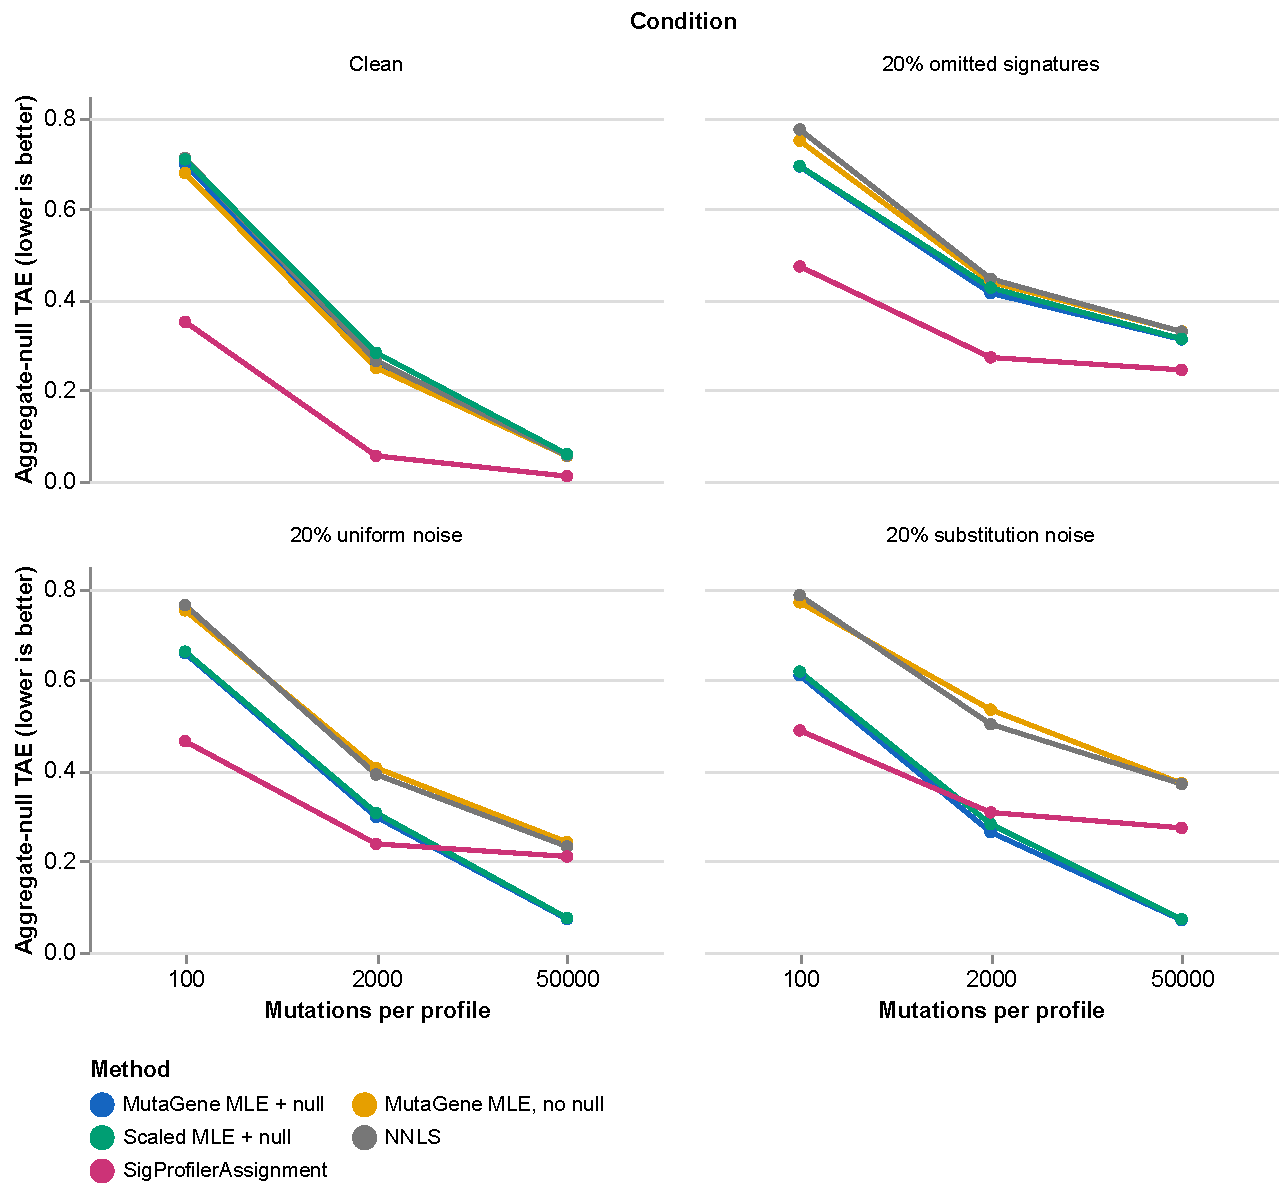
\includegraphics[width=.9\linewidth]{../analysis/signature-benchmark-2026/figures/attribution.pdf}
\caption{Mean attribution error across burdens and controls. Each point summarizes 400 profiles. The report provides paired, cancer-stratified bootstrap intervals.}
\label{fig:benchmark}
\end{figure}

\subsection{Comparator performance and numerical stability}
SigProfilerAssignment achieves lower mean error for clean and omitted-signature conditions at every tested burden.
At 2,000 mutations, clean-data error is 0.056, compared with 0.259 for baseline MLE with null signatures.
At 50,000 mutations, known-signature F1 is 0.982 versus 0.310, respectively.
MutaGene achieves slightly higher reconstruction similarity despite its less accurate attribution.
This difference illustrates over-attribution among correlated signatures.

The baseline optimizer reports failure in 68.1\% of null-enabled fits at 50,000 mutations across all four conditions.
Its fallback returns normalized NNLS estimates.
The scaled-MLE ablation converges in all 4,800 profiles and reduces measured fitting time substantially.
However, it does not consistently reduce attribution error.
The implementation therefore exposes it as an experimental option and reports optimizer diagnostics.
The default fitting objective remains unchanged.

\section{Interpretation and limitations}
This assessment supports method comparison by intended use rather than a universal ranking.
The noise controls deliberately match structures that the null basis can represent.
They do not establish robustness to sequencing artifacts, arbitrary background processes, or real omitted biology.
The clean and omitted-signature results support an optional SigProfilerAssignment workflow.
They do not establish its superiority across all catalogs, cancer types, or assay designs.

The benchmark uses synthetic counts and empirical exposure distributions, not newly adjudicated patient-level truth.
It holds the cancer panel and references fixed.
Its paired bootstrap intervals describe Monte Carlo variation conditional on these distributions.
They do not estimate uncertainty across all cancer populations.
Clinical interpretation requires independent validation and appropriate mutation opportunities.
The software changes do not validate additional driver discoveries or clinical utility.

Recent methods broaden the comparison space.
MuSiCal addresses robust signature discovery and attribution~\cite{musical}.
BASCULE integrates biological priors and multiple signature types~\cite{bascule}.
MutaPheno emphasizes interpretable molecular features for driver-mutation prediction~\cite{mutapheno}.
We cite these developments as context and do not infer unmeasured improvements for MutaGene.

\section{Availability and review requirements}
The source repository is \url{https://github.com/neksa/mutagene}.
This draft describes local changes on the \texttt{feature/adoption-benchmark-2026} branch.
It does not claim that PyPI or the public website contains these changes.
The evidence bundle includes a Quarto report, Vega-Lite specifications, tabular metrics, and reproducible runners.
The AlphaMissense cache remains external to Git because its canonical tables exceed 600 MB.
Its provenance identifies the CC-BY-4.0 Zenodo record 10813168.

Before submission, the authors must confirm authorship, affiliations, funding, competing interests, and data-availability wording.
They must also select an archival release and review third-party data redistribution terms.
The draft requires independent scientific review before bioRxiv submission.

{\small
\begin{thebibliography}{99}
\setlength{\itemsep}{2pt}
\bibitem{mutagene} Goncearenco A et al. Exploring background mutational processes to decipher cancer genetic heterogeneity. \emph{Nucleic Acids Research} (2017). \href{https://doi.org/10.1093/nar/gkx367}{doi:10.1093/nar/gkx367}.
\bibitem{ranking} Brown AL et al. Finding driver mutations in cancer: elucidating the role of background mutational processes. \emph{PLoS Computational Biology} (2019). \href{https://doi.org/10.1371/journal.pcbi.1006981}{doi:10.1371/journal.pcbi.1006981}.
\bibitem{patterns} Manders F et al. MutationalPatterns: the one stop shop for the analysis of mutational processes. \emph{BMC Genomics} (2022). \href{https://doi.org/10.1186/s12864-022-08357-3}{doi:10.1186/s12864-022-08357-3}.
\bibitem{alphamissense} Cheng J et al. Accurate proteome-wide missense variant effect prediction with AlphaMissense. \emph{Science} (2023). \href{https://doi.org/10.1126/science.adg7492}{doi:10.1126/science.adg7492}.
\bibitem{canceram} Ostroverkhova D, Sheng Y, Panchenko AR. Are Next-Generation Pathogenicity Predictors Applicable to Cancer? \emph{Journal of Molecular Biology} (2024). \href{https://doi.org/10.1016/j.jmb.2024.168644}{doi:10.1016/j.jmb.2024.168644}.
\bibitem{benchmark2024} Medo M, Ng CKY, Medova M. A comprehensive comparison of tools for fitting mutational signatures. \emph{Nature Communications} (2024). \href{https://doi.org/10.1038/s41467-024-53711-6}{doi:10.1038/s41467-024-53711-6}.
\bibitem{spa} D\'{i}az-Gay M et al. Assigning mutational signatures to individual samples and individual somatic mutations with SigProfilerAssignment. \emph{Bioinformatics} (2023). \href{https://doi.org/10.1093/bioinformatics/btad756}{doi:10.1093/bioinformatics/btad756}.
\bibitem{benchmark2025} Jiang N, Wu Y, Rozen SG. Benchmarking 13 tools for mutational signature attribution, including a new and improved algorithm. \emph{Briefings in Bioinformatics} (2025). \href{https://doi.org/10.1093/bib/bbaf042}{doi:10.1093/bib/bbaf042}.
\bibitem{musical} Jin H et al. Accurate and sensitive mutational signature analysis with MuSiCal. \emph{Nature Genetics} (2024). \href{https://doi.org/10.1038/s41588-024-01659-0}{doi:10.1038/s41588-024-01659-0}.
\bibitem{bascule} Buscaroli E et al. BASCULE: bayesian inference and clustering of mutational signatures leveraging biological priors. \emph{Genome Biology} (2026). \href{https://doi.org/10.1186/s13059-025-03835-9}{doi:10.1186/s13059-025-03835-9}.
\bibitem{mutapheno} Yang Y et al. An interpretable molecular framework for predicting cancer driver missense mutations. \emph{Proceedings of the National Academy of Sciences} (2026). \href{https://doi.org/10.1073/pnas.2524289123}{doi:10.1073/pnas.2524289123}.
\end{thebibliography}
}
\end{document}
